\pagebreak
\chapter*{Usage}

\begin{figure}[H]
\centering
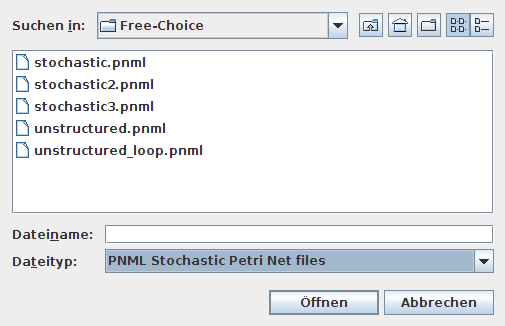
\includegraphics[width=0.6\textwidth]{import.png}
\caption{Importing stochastic Petri nets stored in .pnml-format}
\label{fig:import_dialog}
\end{figure}

\section*{Load an existing annotated PNML file}
You can just click on the import\ldots~button on the top right corner of the ProM workbench and select a \texttt{.pnml} file with a stochastic Petri net, cf. Fig.~\ref{fig:import_dialog}.
The stochastic extension is added as a \texttt{<toolspecific>} annotation to each transition. An example \emph{immediate} transition could look like this:

\lstset{language=XML}
\begin{lstlisting}
    <transition id="tr4">
        <name>
          <text>t_start</text>
        </name>
        <graphics>
          <position x="59" y="92" />
          <dimension x="10" y="32" />
        </graphics>
	<toolspecific tool="StochasticPetriNet" version="0.1">
	  <property key="priority">1</property>
	  <property key="weight">1</property>
      	  <property key="distributionType">IMMEDIATE</property>
          <property key="distributionParameters"></property>
        </toolspecific>
      </transition>
\end{lstlisting}
Note that the \texttt{tool}-attribute needs to be set to \texttt{"StochasticPetriNet"}
 
The annotated properties for transitions are:
\begin{itemize}
  \item the \emph{priority} of the transition. Semantics: of all enabled transitions, only the transitions with highest priority may fire. Immediate transitions have \emph{priority} $\geq$ 1, whereas timed transitions have \emph{priority} = 0.  
  \item the \emph{weight} of the transition. Used for probabilistic choice between two or more immediate transitions. Each transition will be used proportionally often as their weight is in relation to the whole weight of all enabled transitions.
  \item the \emph{distributionType} is used to specify which parametric/non-parametric type the timed transition has, or if it is an \texttt{IMMEDIATE} transition. For timed transitions, following distribution types are supported:
  \begin{itemize}
    \item BETA
    \item EXPONENTIAL
    \item NORMAL
    \item LOGNORMAL
    \item GAMMA
    \item UNIFORM
    \item WEIBULL
    \item GAUSSIAN\_KERNEL
    \item HISTOGRAM
    \item LOG\_SPLINE (optional, only powered with R-support) 
  \end{itemize}
  \item the \emph{distributionParameters} contains a semicolon \texttt{;} separated list of double values. The number of parameters depends on the type of the distribution. For example, the \texttt{NORMAL} distribution needs two parameters: $\mu$ mean, and $\sigma$ standard deviation.
  The \texttt{EXPONENTIAL} distribution only needs one parameter: $\lambda$ the firing rate.
  Nonparametric methods like the gaussian kernel density estimator store all sample values separated by a semicolon.
\end{itemize}

\section*{Enrich Petri net by manual replay using \emph{Replay PN for Performance analysis}}
If no stochastically enriched \texttt{.pnml}-file exists yet, you can enrich an existing petri net with performance data gathered from a log. 
Therefore, replay the log in the model for performance analysis (PNetReplayer plugin) and obtain \emph{Manifest}
Use the \emph{Manifest} as input to the plugin \texttt{Enrich Petri net with performance data}

\subsection*{Prerequisites}
\begin{compactitem}
  \item load a Log file with timestamp attributes.
  \item a fitting Petri net model that can be mapped to the log file.
  (try either mining algorithms, or model it yourself with e.g. Yasper, or CPNTools.)  
\end{compactitem} 

\begin{figure}[H]
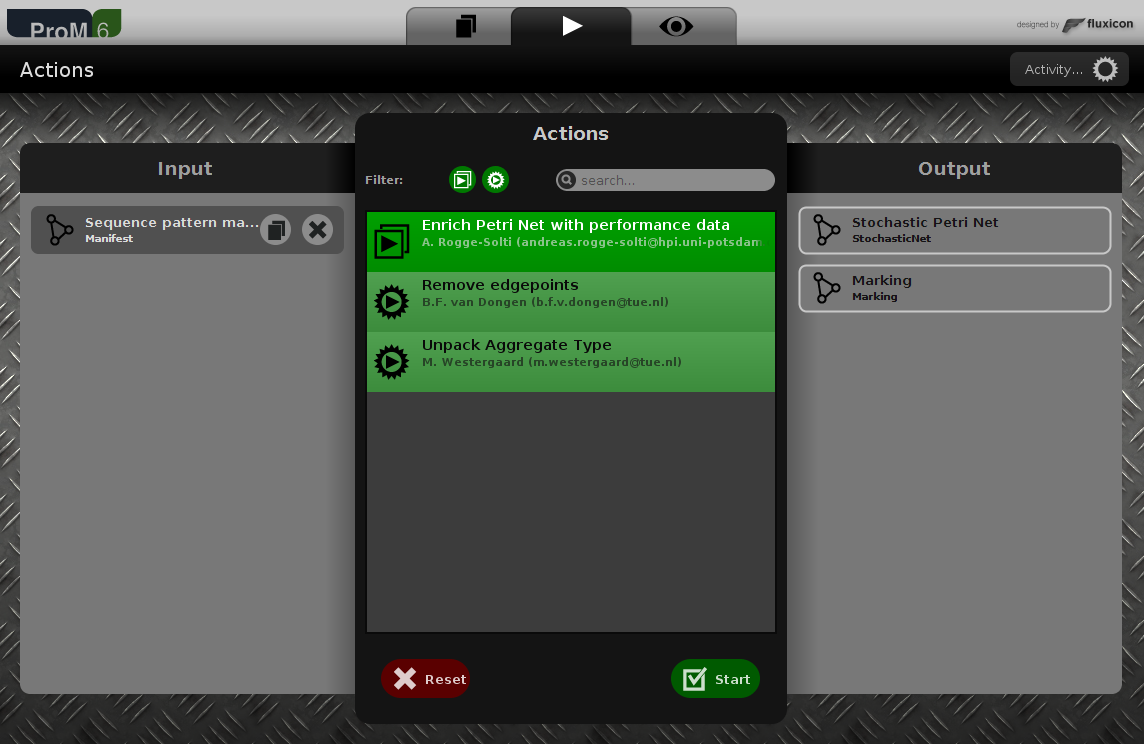
\includegraphics[width=\textwidth]{enrich2_1.png}
\caption{Convert a replayed Log and Petri net (Manifest) to a StochasticNet}
\label{fig:convert_manifest}
\end{figure}

\subsection*{Type of distributions}
Select the kind of distributions that shall be used in the stochastic Petri net: (Fig.~\ref{fig:distribution_type_selection})
\begin{figure}[h]
\centering
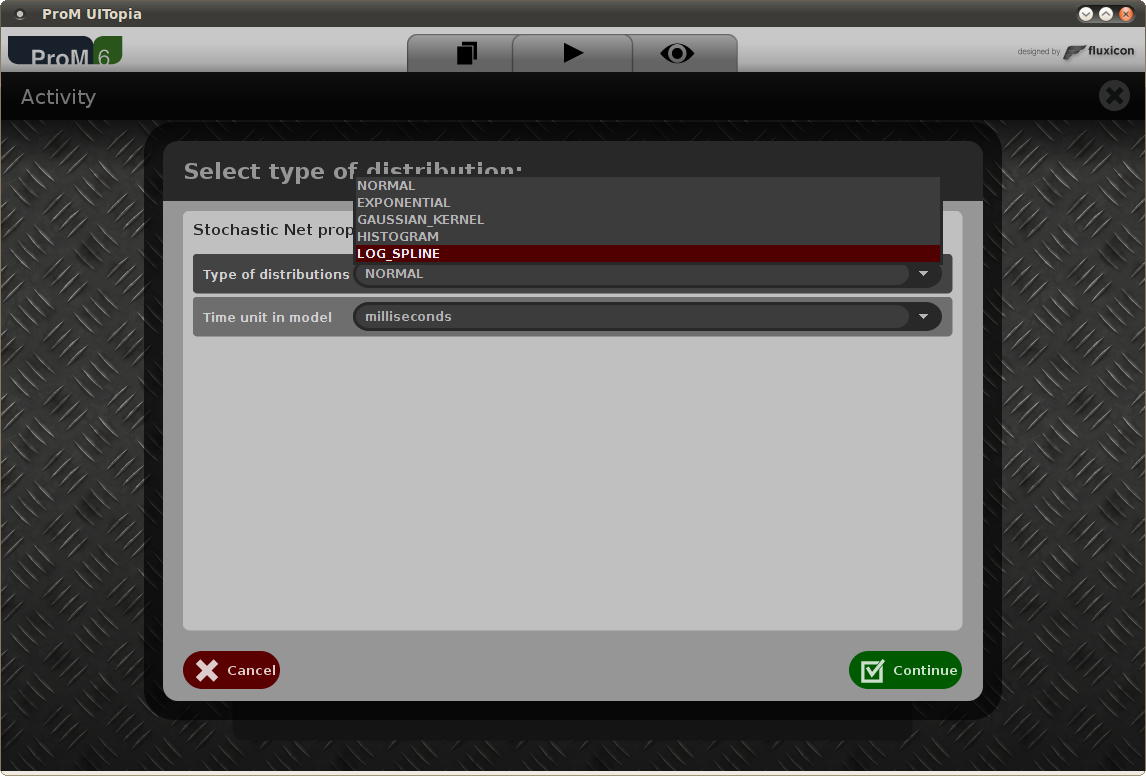
\includegraphics[width=0.85\textwidth]{enrich1_2.png}
\caption{Select the type of the distributions at timed transitions}
\label{fig:distribution_type_selection}
\end{figure}

\begin{compactitem}
  \item The \texttt{NORMAL} type assumes normally distributed transition durations, and collects means and standard deviations of the historical activity durations.
  \item The \texttt{EXPONENTIAL} type assumes exponetially distributed delays for transition durations and uses the observed sample means as parameter for exponential activity durations.
  \item The \texttt{GAUSSIAN\_KERNEL} type performs a kernel density fit with Gaussian kernels, cf. Fig.~\ref{fig:gauss_kernel}
  \item The \texttt{HISTOGRAM} type creates simple histograms for visualization.
  \item The \texttt{LOG\_SPLINE} type is only available, if you installed \texttt{R} correctly, cf. Sect.~\ref{sec:Installation}
\end{compactitem} 

\subsection*{Time unit in model}
You can select the unit of the parametric models. This unit will influence also the bin-size of the \texttt{HISTOGRAM} distribution type.

\section*{Enrich Petri net by automatic replay using default mapping by name}
If your Petri net model that you want to enrich corresponds to the log, such that the transition names are equal, and each visible transition has corresponding events, you can save yourself the wizard of the \emph{Replay Petri net for performance analysis} plugin and use Log and Petri net model directly as input to the \emph{Enrich Petri net with performance data (default mapping)} plugin.


\section*{Visualize the stochastic Petri net}
Once you have loaded a stochastic Petri net successfully, or you managed to enrich a Petri net with performance data from a Log,
you can view it. Open the \emph{Stochastic Petri Net Visualizer}, as shown in Fig.~\ref{fig:open_visualizer}

\begin{figure}[H]
\centering
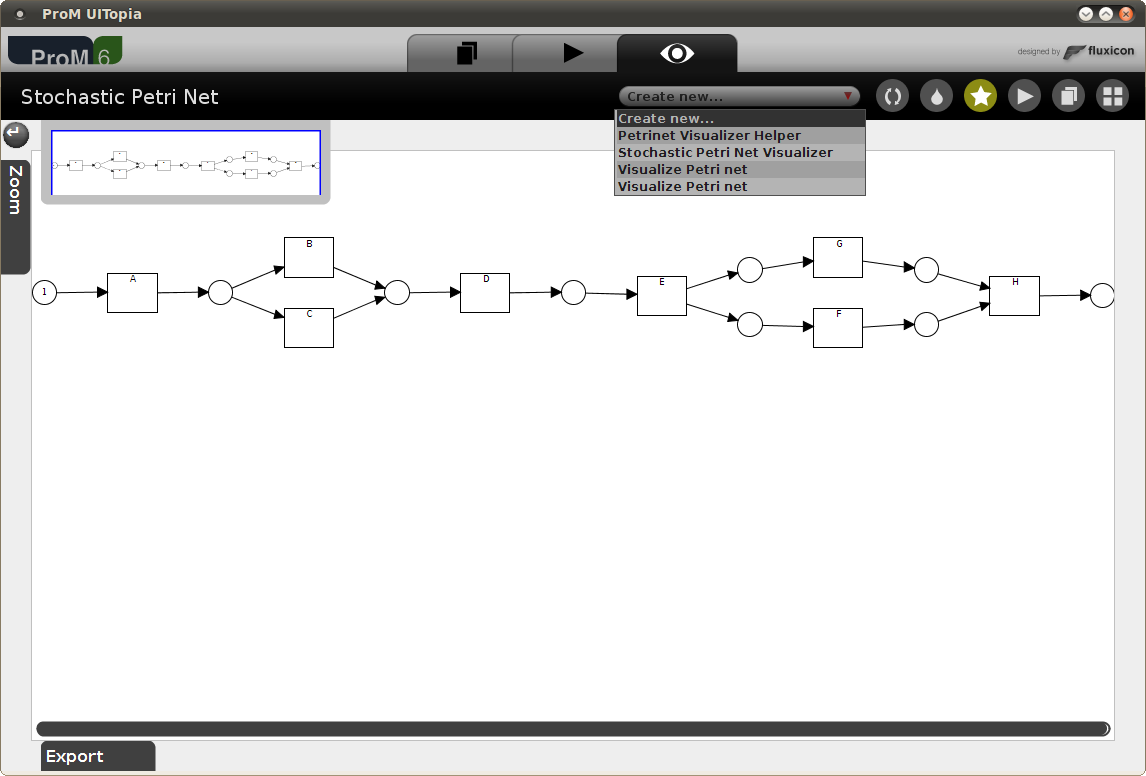
\includegraphics[width=0.95\textwidth]{visualize.png}
\caption{Select the \texttt{Stochastic Petri Net Visualizer} to see the stochastic annotations.}
\label{fig:open_visualizer}
\end{figure}

\begin{figure}[H]
\centering
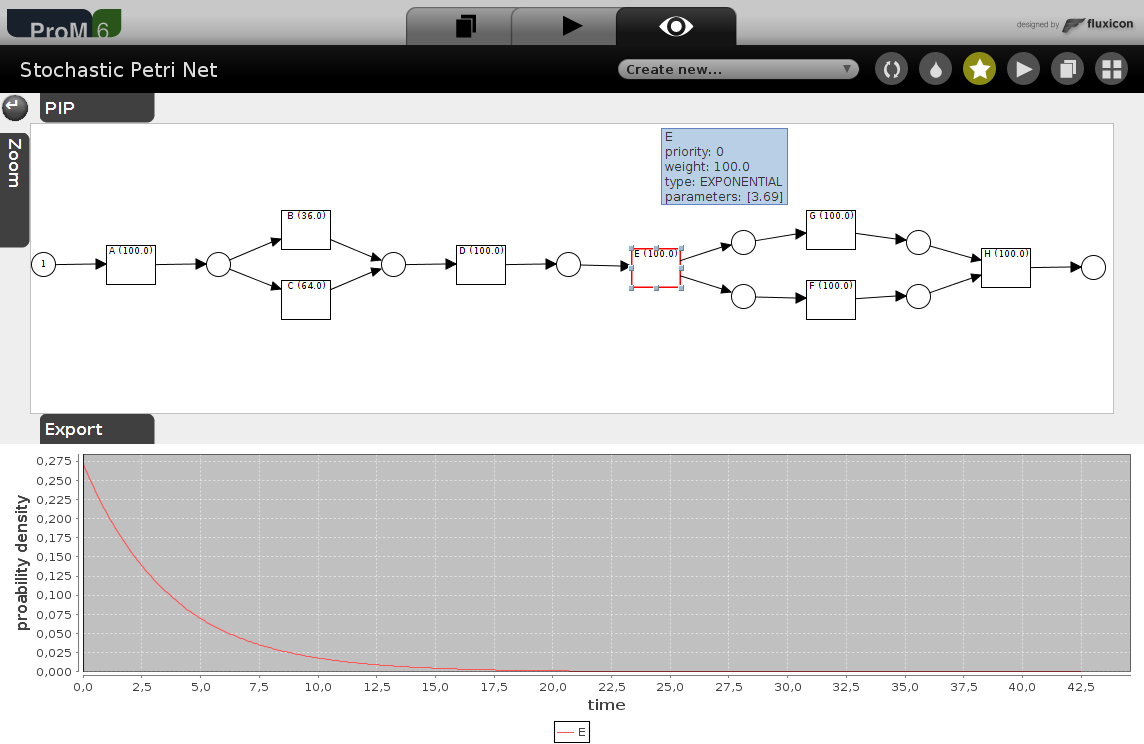
\includegraphics[width=0.95\textwidth]{visualize2.png}
\caption{Exponential distributions -- fit to the observed mean durations.}
\label{fig:exponential_distributions}
\end{figure}

\begin{figure}[H]
\centering
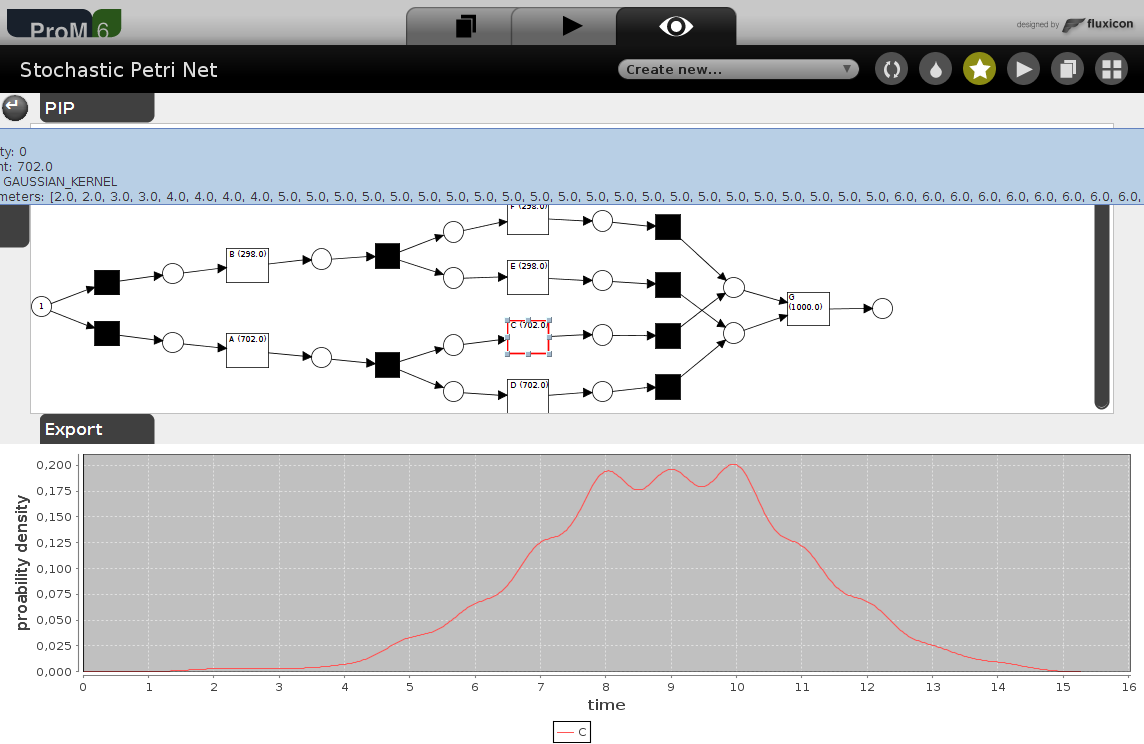
\includegraphics[width=0.95\textwidth]{visualize2_gaussian_kernel.png}
\caption{Activity duration densities obtained from the observed data. Fit by kernel density regression with Gaussian kernels.}
\label{fig:gauss_kernel}
\end{figure}

\begin{figure}[H]
\centering
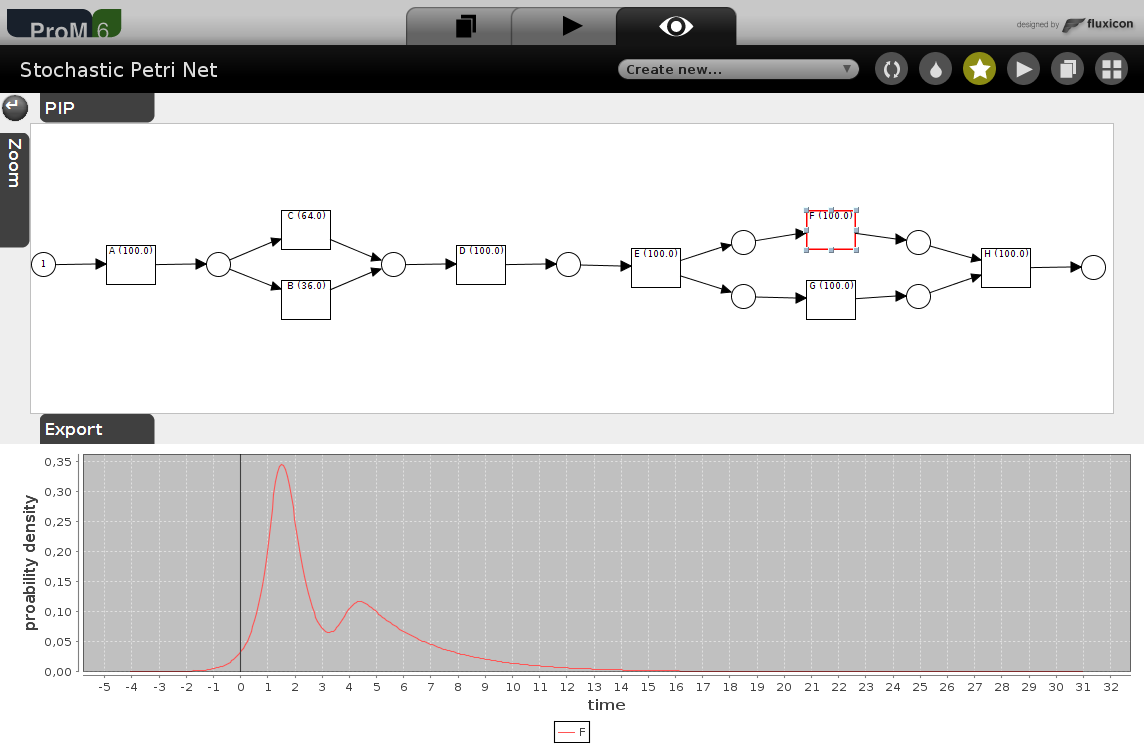
\includegraphics[width=0.95\textwidth]{visualize2_logspline.png}
\caption{Log-Spline distributions.}
\label{fig:log-spline_distributions}
\end{figure}